\chapter{Related Work}\label{chapter:relatedwork}
\begin{figure*}[t]
    \centering
	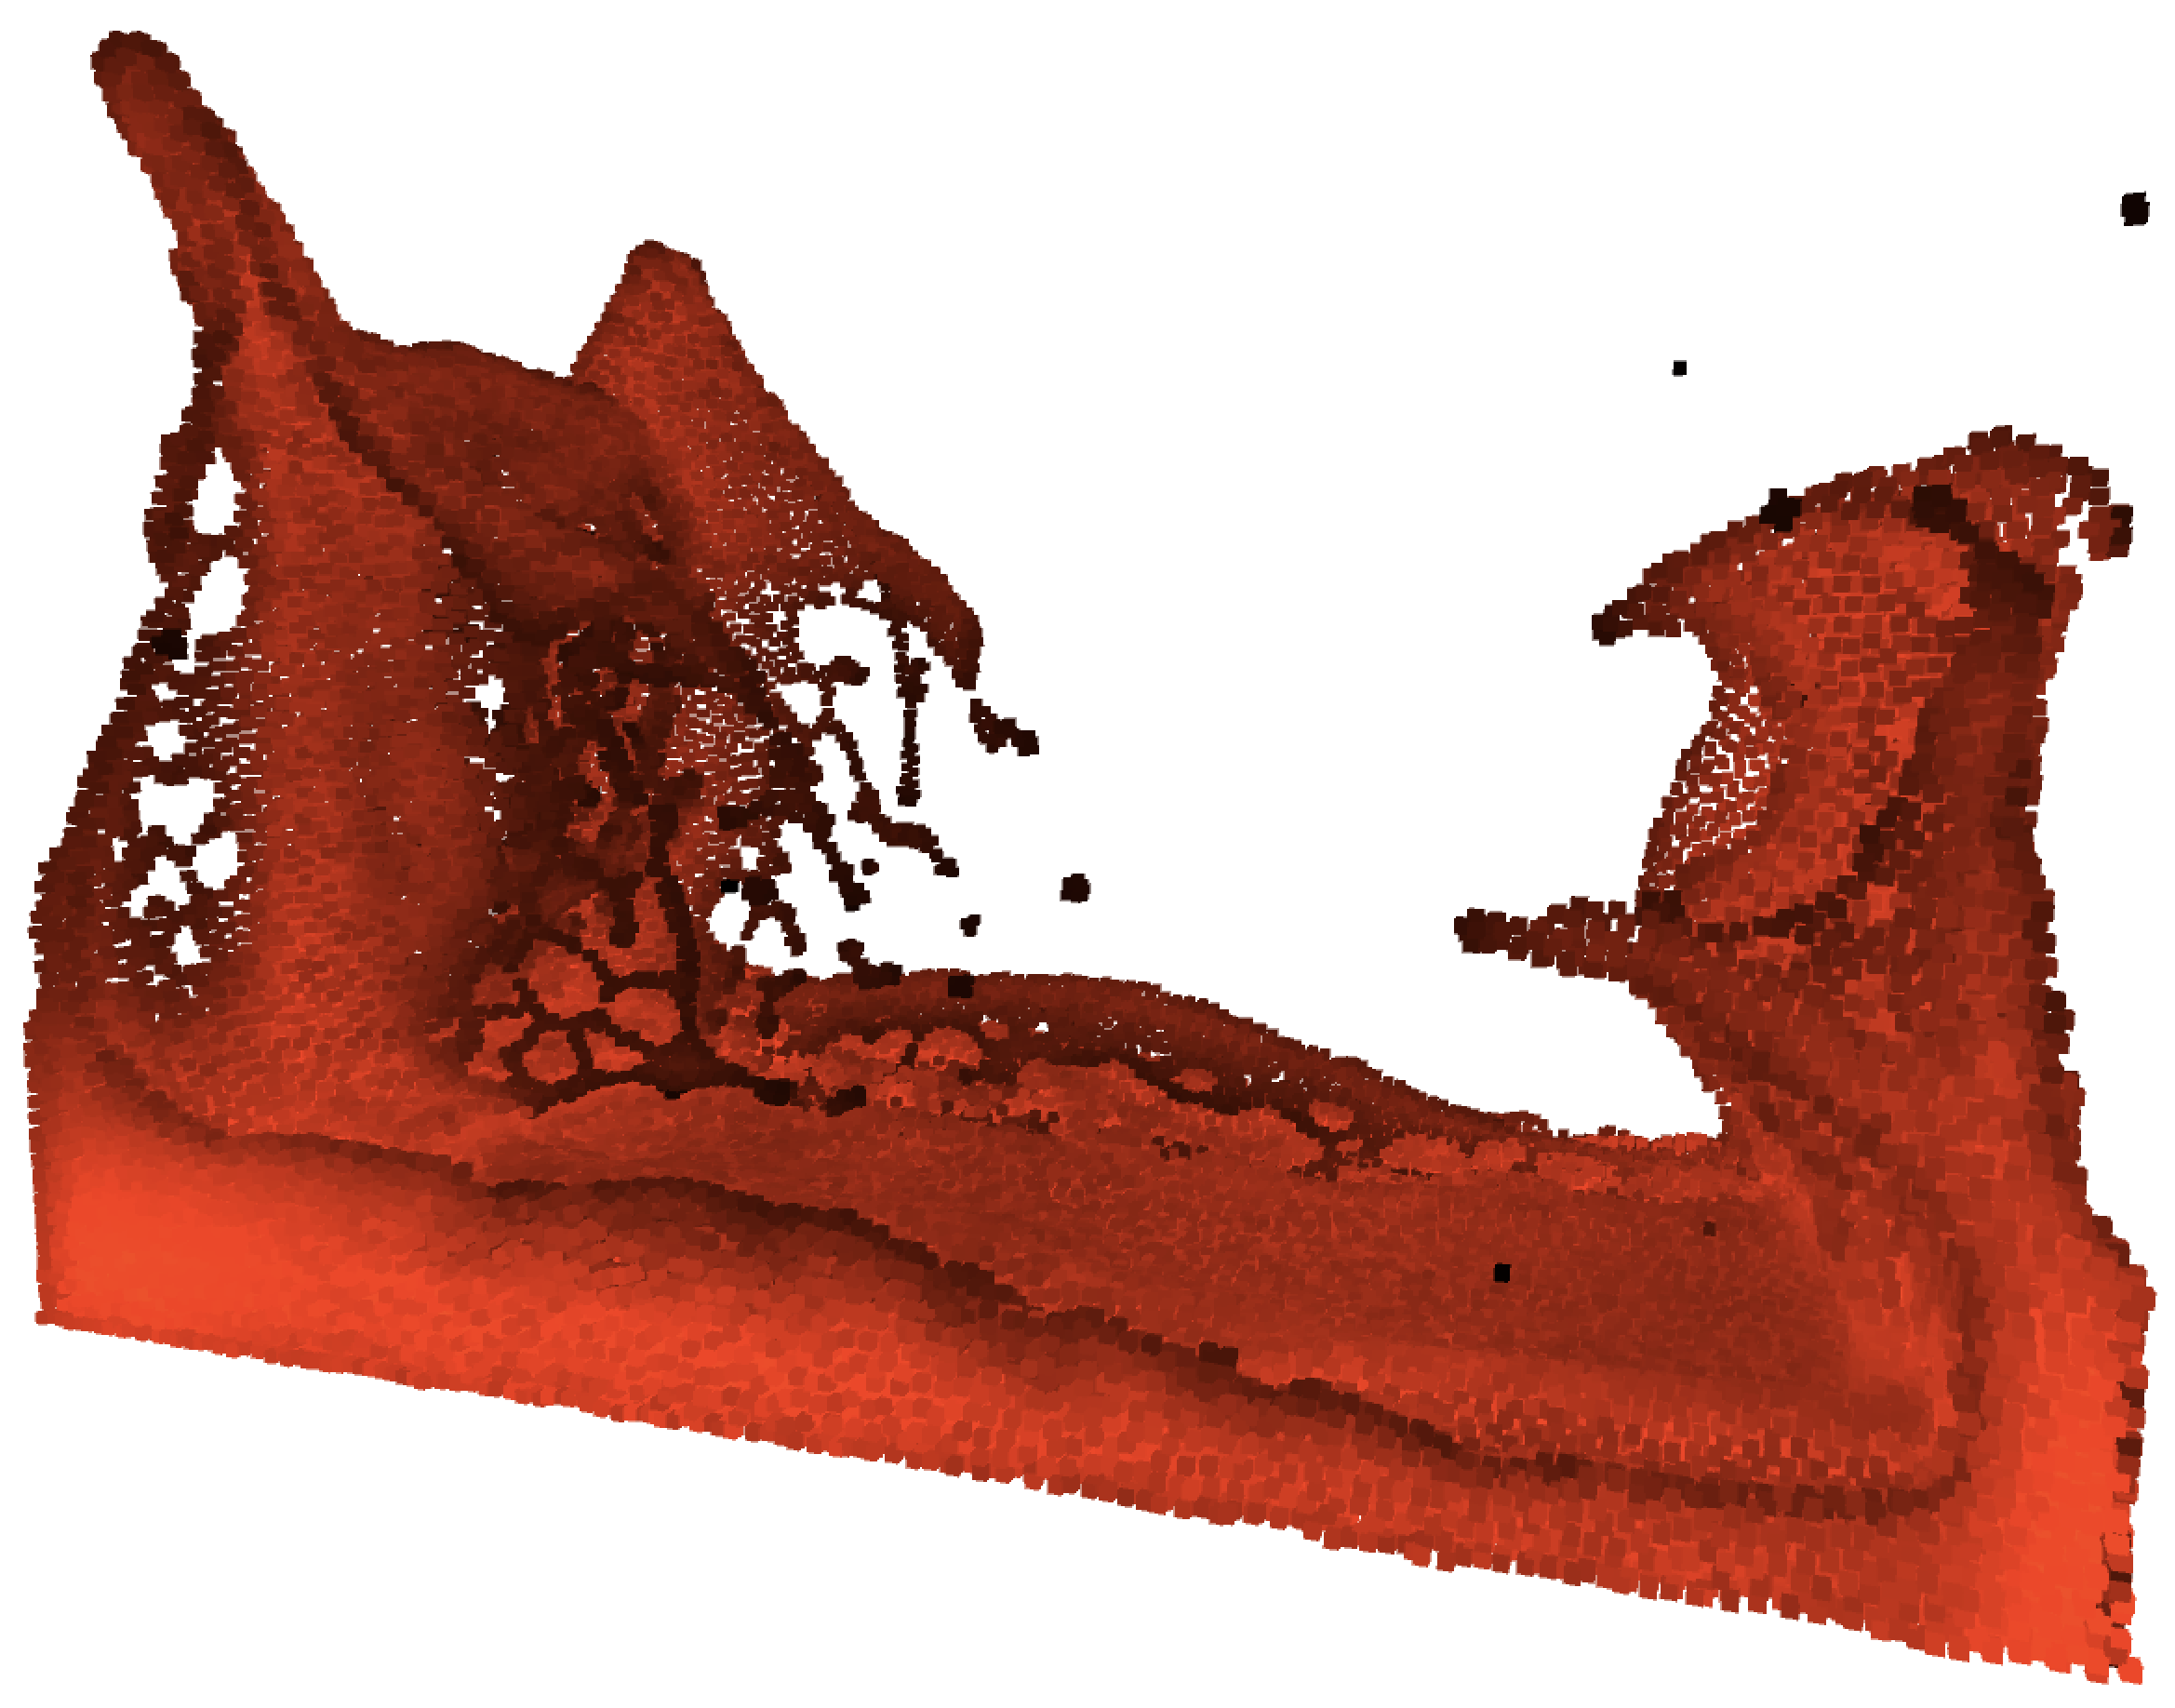
\includegraphics[scale=0.35]{figures/unity-sph2}

	\caption{Particle-based fluid simulation in Unity3D \parencite{unity3d} \parencite{mysph}}
\end{figure*}


Computational Fluid Dynamics (CFD) has been a research topic long before the first computers appeared. Based on Newton's Second Law, Leonard Euler developed a mathematical model to describe the flow of frictionless inviscid fluids by a set of differential equations in 1757 \parencite{euler1757principes}. Claude Navier and George Stokes extended the Euler Equations by a Viscosity term and formulated the Navier-Stokes-Equations. \\\\
In computer graphics two distinctive approaches have established to numerically approximate the Navier-Stokes-Equations: 
\par The Lagragian methods use particles to represent a fluid. The Smoothed Particle Hydrodynamics (SPH) method was presented by Lucy in 1977 to simulate astrophysical problems \parencite{lucy1977numerical}. In 1992 Monaghan applied the SPH method to fluid dynamics by approximating continuous velocity flow-fields of the Navier-Stokes-Equations using particles with discrete positions and velocities \parencite{monaghan1992smoothed}. SPH particles are advected by exerting pressure, viscosity and/or surface tension forces on each other using smoothing kernels \parencite{muller2003particle}. However, it does not fulfill the incompressibility constraint, which can cause undesired visual artifacts. Becker and Teschner presented the weakly compressible SPH system (WCSPH) to maintain incompressibility with the cost of limiting the time-step to impractical sizes \parencite{becker2007weakly}. Macklin and Mueller introduced Position Based Fluids (PBF) which first advects particles and then corrects its positions to satisfy the incompressibility conditions iteratively \parencite{macklin2013position}. Several improvements had been done since then and it is still an active topic in research (TODO papers) \parencite{morikawaimprovements}.
\par The alternative to particle-based approaches is the Eulerian viewpoint that splits continuous quantities on a discrete regular grid. First described by Harlow and Welch in 1965 \parencite{harlow1965numerical}, they presented the Marker-and-Cell (MAC) grid to prevent biased or null-spaced central differences when advecting velocities. Incompressibility in grid-based approaches is enforced by solving the pressure Poisson equation with a divergence-free velocity field. [TODO: Smth. about CG]
\par Compared to particle-based approaches the grid-based approach achieve higher accuracy. Particle-based methods only needs computation where particles are; the grid-based method always considers to whole grid. This makes the particle-based viewpoint more suitable for simulations in which the fluid moves through an open domain environment like for example in games. 
\par In the recent years Deep Learning emerged in many fields of research, because GPUs far surpassed the computational capabilities needed to train Neural Networks of multicore CPUs \parencite{raina2009large}. Deep Neural Networks learn patterns in large data sets by using the backpropagation algorithm and dramatically improved the state-of-the-art in speech recognition, visual object recognition, object detection and many other domains \parencite{lecun2015deep}. Furthermore several recent papers have targeted to use NNs to mimic physical phenomena like rigid-body simulations \parencite{chang2016compositional} and also fluid dynamics \parencite{tompson2017accelerating}  \parencite{chu2017data} \parencite{schenck2018spnets}. Those approaches benefit from the fact, that the evaluation and thus simulation of those NNs are much faster than the conventional mathematical approaches.